% Options for packages loaded elsewhere
\PassOptionsToPackage{unicode}{hyperref}
\PassOptionsToPackage{hyphens}{url}
%
\documentclass[
]{article}
\usepackage{amsmath,amssymb}
\usepackage{iftex}
\ifPDFTeX
  \usepackage[T1]{fontenc}
  \usepackage[utf8]{inputenc}
  \usepackage{textcomp} % provide euro and other symbols
\else % if luatex or xetex
  \usepackage{unicode-math} % this also loads fontspec
  \defaultfontfeatures{Scale=MatchLowercase}
  \defaultfontfeatures[\rmfamily]{Ligatures=TeX,Scale=1}
\fi
\usepackage{lmodern}
\ifPDFTeX\else
  % xetex/luatex font selection
\fi
% Use upquote if available, for straight quotes in verbatim environments
\IfFileExists{upquote.sty}{\usepackage{upquote}}{}
\IfFileExists{microtype.sty}{% use microtype if available
  \usepackage[]{microtype}
  \UseMicrotypeSet[protrusion]{basicmath} % disable protrusion for tt fonts
}{}
\makeatletter
\@ifundefined{KOMAClassName}{% if non-KOMA class
  \IfFileExists{parskip.sty}{%
    \usepackage{parskip}
  }{% else
    \setlength{\parindent}{0pt}
    \setlength{\parskip}{6pt plus 2pt minus 1pt}}
}{% if KOMA class
  \KOMAoptions{parskip=half}}
\makeatother
\usepackage{xcolor}
\usepackage[margin=1in]{geometry}
\usepackage{color}
\usepackage{fancyvrb}
\newcommand{\VerbBar}{|}
\newcommand{\VERB}{\Verb[commandchars=\\\{\}]}
\DefineVerbatimEnvironment{Highlighting}{Verbatim}{commandchars=\\\{\}}
% Add ',fontsize=\small' for more characters per line
\usepackage{framed}
\definecolor{shadecolor}{RGB}{248,248,248}
\newenvironment{Shaded}{\begin{snugshade}}{\end{snugshade}}
\newcommand{\AlertTok}[1]{\textcolor[rgb]{0.94,0.16,0.16}{#1}}
\newcommand{\AnnotationTok}[1]{\textcolor[rgb]{0.56,0.35,0.01}{\textbf{\textit{#1}}}}
\newcommand{\AttributeTok}[1]{\textcolor[rgb]{0.13,0.29,0.53}{#1}}
\newcommand{\BaseNTok}[1]{\textcolor[rgb]{0.00,0.00,0.81}{#1}}
\newcommand{\BuiltInTok}[1]{#1}
\newcommand{\CharTok}[1]{\textcolor[rgb]{0.31,0.60,0.02}{#1}}
\newcommand{\CommentTok}[1]{\textcolor[rgb]{0.56,0.35,0.01}{\textit{#1}}}
\newcommand{\CommentVarTok}[1]{\textcolor[rgb]{0.56,0.35,0.01}{\textbf{\textit{#1}}}}
\newcommand{\ConstantTok}[1]{\textcolor[rgb]{0.56,0.35,0.01}{#1}}
\newcommand{\ControlFlowTok}[1]{\textcolor[rgb]{0.13,0.29,0.53}{\textbf{#1}}}
\newcommand{\DataTypeTok}[1]{\textcolor[rgb]{0.13,0.29,0.53}{#1}}
\newcommand{\DecValTok}[1]{\textcolor[rgb]{0.00,0.00,0.81}{#1}}
\newcommand{\DocumentationTok}[1]{\textcolor[rgb]{0.56,0.35,0.01}{\textbf{\textit{#1}}}}
\newcommand{\ErrorTok}[1]{\textcolor[rgb]{0.64,0.00,0.00}{\textbf{#1}}}
\newcommand{\ExtensionTok}[1]{#1}
\newcommand{\FloatTok}[1]{\textcolor[rgb]{0.00,0.00,0.81}{#1}}
\newcommand{\FunctionTok}[1]{\textcolor[rgb]{0.13,0.29,0.53}{\textbf{#1}}}
\newcommand{\ImportTok}[1]{#1}
\newcommand{\InformationTok}[1]{\textcolor[rgb]{0.56,0.35,0.01}{\textbf{\textit{#1}}}}
\newcommand{\KeywordTok}[1]{\textcolor[rgb]{0.13,0.29,0.53}{\textbf{#1}}}
\newcommand{\NormalTok}[1]{#1}
\newcommand{\OperatorTok}[1]{\textcolor[rgb]{0.81,0.36,0.00}{\textbf{#1}}}
\newcommand{\OtherTok}[1]{\textcolor[rgb]{0.56,0.35,0.01}{#1}}
\newcommand{\PreprocessorTok}[1]{\textcolor[rgb]{0.56,0.35,0.01}{\textit{#1}}}
\newcommand{\RegionMarkerTok}[1]{#1}
\newcommand{\SpecialCharTok}[1]{\textcolor[rgb]{0.81,0.36,0.00}{\textbf{#1}}}
\newcommand{\SpecialStringTok}[1]{\textcolor[rgb]{0.31,0.60,0.02}{#1}}
\newcommand{\StringTok}[1]{\textcolor[rgb]{0.31,0.60,0.02}{#1}}
\newcommand{\VariableTok}[1]{\textcolor[rgb]{0.00,0.00,0.00}{#1}}
\newcommand{\VerbatimStringTok}[1]{\textcolor[rgb]{0.31,0.60,0.02}{#1}}
\newcommand{\WarningTok}[1]{\textcolor[rgb]{0.56,0.35,0.01}{\textbf{\textit{#1}}}}
\usepackage{graphicx}
\makeatletter
\def\maxwidth{\ifdim\Gin@nat@width>\linewidth\linewidth\else\Gin@nat@width\fi}
\def\maxheight{\ifdim\Gin@nat@height>\textheight\textheight\else\Gin@nat@height\fi}
\makeatother
% Scale images if necessary, so that they will not overflow the page
% margins by default, and it is still possible to overwrite the defaults
% using explicit options in \includegraphics[width, height, ...]{}
\setkeys{Gin}{width=\maxwidth,height=\maxheight,keepaspectratio}
% Set default figure placement to htbp
\makeatletter
\def\fps@figure{htbp}
\makeatother
\setlength{\emergencystretch}{3em} % prevent overfull lines
\providecommand{\tightlist}{%
  \setlength{\itemsep}{0pt}\setlength{\parskip}{0pt}}
\setcounter{secnumdepth}{-\maxdimen} % remove section numbering
\ifLuaTeX
  \usepackage{selnolig}  % disable illegal ligatures
\fi
\usepackage{bookmark}
\IfFileExists{xurl.sty}{\usepackage{xurl}}{} % add URL line breaks if available
\urlstyle{same}
\hypersetup{
  pdftitle={Direct Approach KEF},
  pdfauthor={Pouya Roudaki},
  hidelinks,
  pdfcreator={LaTeX via pandoc}}

\title{Direct Approach KEF}
\author{Pouya Roudaki}
\date{2024-10-21}

\begin{document}
\maketitle

\section{Kernel Mean Embedding
Estimation}\label{kernel-mean-embedding-estimation}

\begin{Shaded}
\begin{Highlighting}[]
\FunctionTok{setwd}\NormalTok{(}\StringTok{"C:/Users/rouda/OneDrive/Research/Codes/R/kef"}\NormalTok{)}
\FunctionTok{getwd}\NormalTok{()  }\CommentTok{\# Confirm it points to the package root}
\end{Highlighting}
\end{Shaded}

\begin{verbatim}
## [1] "C:/Users/rouda/OneDrive/Research/Codes/R/kef"
\end{verbatim}

\begin{Shaded}
\begin{Highlighting}[]
\NormalTok{devtools}\SpecialCharTok{::}\FunctionTok{install}\NormalTok{(}\StringTok{"."}\NormalTok{)}
\end{Highlighting}
\end{Shaded}

\begin{verbatim}
## -- R CMD build -----------------------------------------------------------------
##       v  checking for file 'C:\Users\rouda\OneDrive\Research\Codes\R\kef/DESCRIPTION'
##       -  preparing 'kef':
##    checking DESCRIPTION meta-information ...  v  checking DESCRIPTION meta-information
##       -  checking for LF line-endings in source and make files and shell scripts
##   -  checking for empty or unneeded directories
##      Omitted 'LazyData' from DESCRIPTION
##      NB: this package now depends on R (>=        NB: this package now depends on R (>= 3.5.0)
##        WARNING: Added dependency on R >= 3.5.0 because serialized objects in
##      serialize/load version 3 cannot be read in older versions of R.
##      File(s) containing such objects:
##        'kef/examples/rdata_direct.RData' 'kef/examples/rdata_direct_1.RData'
##        'kef/examples/rdata_direct_2.RData'
##        'kef/examples/rdata_direct_4.RData'
##      'kef/examples/rdata_direct_brownian_1.RData'         'kef/examples/rdata_direct_brownian_1.RData'
## -  building 'kef_0.1.0.tar.gz'
##      
## Running "C:/PROGRA~1/R/R-43~1.1/bin/x64/Rcmd.exe" INSTALL \
##   "C:\Users\rouda\AppData\Local\Temp\RtmpC2C1PZ/kef_0.1.0.tar.gz" \
##   --install-tests 
## * installing to library 'C:/Users/rouda/AppData/Local/R/win-library/4.3'
## * installing *source* package 'kef' ...
## ** using staged installation
## ** R
## ** byte-compile and prepare package for lazy loading
## Warning: package 'pracma' was built under R version 4.3.3
## Note: possible error in 'norm(s, type = "2")': unused argument (type = "2") 
## Note: possible error in 'gram_matrix(vec_list = list_fixed, ': unused argument (centering_param = centering_param) 
## Note: possible error in 'gram_matrix(vec_list = list_fixed, ': unused argument (centering_param = centering_param) 
## ** help
## *** installing help indices
## ** building package indices
## ** testing if installed package can be loaded from temporary location
## ** testing if installed package can be loaded from final location
## ** testing if installed package keeps a record of temporary installation path
## * DONE (kef)
\end{verbatim}

\begin{Shaded}
\begin{Highlighting}[]
\FunctionTok{library}\NormalTok{(}\StringTok{"kef"}\NormalTok{)}
\end{Highlighting}
\end{Shaded}

\begin{verbatim}
## 
## Attaching package: 'kef'
\end{verbatim}

\begin{verbatim}
## The following object is masked from 'package:stats':
## 
##     kernel
\end{verbatim}

\begin{verbatim}
## The following object is masked from 'package:base':
## 
##     norm
\end{verbatim}

\begin{Shaded}
\begin{Highlighting}[]
\FunctionTok{library}\NormalTok{(}\StringTok{"pracma"}\NormalTok{)}
\end{Highlighting}
\end{Shaded}

\begin{verbatim}
## Warning: package 'pracma' was built under R version 4.3.3
\end{verbatim}

\begin{verbatim}
## 
## Attaching package: 'pracma'
\end{verbatim}

\begin{verbatim}
## The following object is masked from 'package:kef':
## 
##     ones
\end{verbatim}

Set the randomness seed.

\begin{Shaded}
\begin{Highlighting}[]
\CommentTok{\# set the seed}

\NormalTok{seed }\OtherTok{\textless{}{-}} \DecValTok{7}
\FunctionTok{set.seed}\NormalTok{(seed)}
\end{Highlighting}
\end{Shaded}

\subsection{Specfiy the True density}\label{specfiy-the-true-density}

Set the mean and standard deviation of normal distribution P

\begin{Shaded}
\begin{Highlighting}[]
\CommentTok{\# Set the mean and standard deviation of normal distribution P}
\NormalTok{ n }\OtherTok{=} \DecValTok{500}
\NormalTok{ means }\OtherTok{=} \FunctionTok{c}\NormalTok{(}\SpecialCharTok{{-}}\DecValTok{2}\NormalTok{, }\DecValTok{2}\NormalTok{)}
\NormalTok{ sds }\OtherTok{=} \FunctionTok{c}\NormalTok{(}\DecValTok{1}\NormalTok{, }\FloatTok{1.5}\NormalTok{)}
\NormalTok{ probabilities }\OtherTok{=} \FunctionTok{c}\NormalTok{(}\FloatTok{0.3}\NormalTok{, }\FloatTok{0.7}\NormalTok{)}
\end{Highlighting}
\end{Shaded}

\subsection{Take Random samples}\label{take-random-samples}

\begin{Shaded}
\begin{Highlighting}[]
\CommentTok{\# vector of fixed points}
\NormalTok{vec\_fixed\_points }\OtherTok{\textless{}{-}} \FunctionTok{sort}\NormalTok{(}\FunctionTok{rnorm\_mixture}\NormalTok{(n, means, sds, probabilities))}

\FunctionTok{library}\NormalTok{(ggplot2)}
\CommentTok{\# Assuming vec\_fixed\_points is your data}
\NormalTok{df }\OtherTok{\textless{}{-}} \FunctionTok{data.frame}\NormalTok{(}\AttributeTok{points =}\NormalTok{ vec\_fixed\_points)}

\CommentTok{\# Create the histogram with 20 breaks}
\FunctionTok{ggplot}\NormalTok{(df, }\FunctionTok{aes}\NormalTok{(}\AttributeTok{x =}\NormalTok{ points, }\AttributeTok{y =}\NormalTok{ ..density..)) }\SpecialCharTok{+}
  \FunctionTok{geom\_histogram}\NormalTok{(}\AttributeTok{bins =} \DecValTok{20}\NormalTok{, }\AttributeTok{fill =} \StringTok{"blue"}\NormalTok{, }\AttributeTok{color =} \StringTok{"black"}\NormalTok{) }\SpecialCharTok{+}
  \FunctionTok{labs}\NormalTok{(}\AttributeTok{title =} \StringTok{"Histogram of sampled points"}\NormalTok{, }\AttributeTok{x =} \StringTok{"Values"}\NormalTok{, }\AttributeTok{y =} \StringTok{"Frequency"}\NormalTok{)}\SpecialCharTok{+}
  \FunctionTok{theme\_bw}\NormalTok{()}
\end{Highlighting}
\end{Shaded}

\begin{verbatim}
## Warning: The dot-dot notation (`..density..`) was deprecated in ggplot2 3.4.0.
## i Please use `after_stat(density)` instead.
## This warning is displayed once every 8 hours.
## Call `lifecycle::last_lifecycle_warnings()` to see where this warning was
## generated.
\end{verbatim}

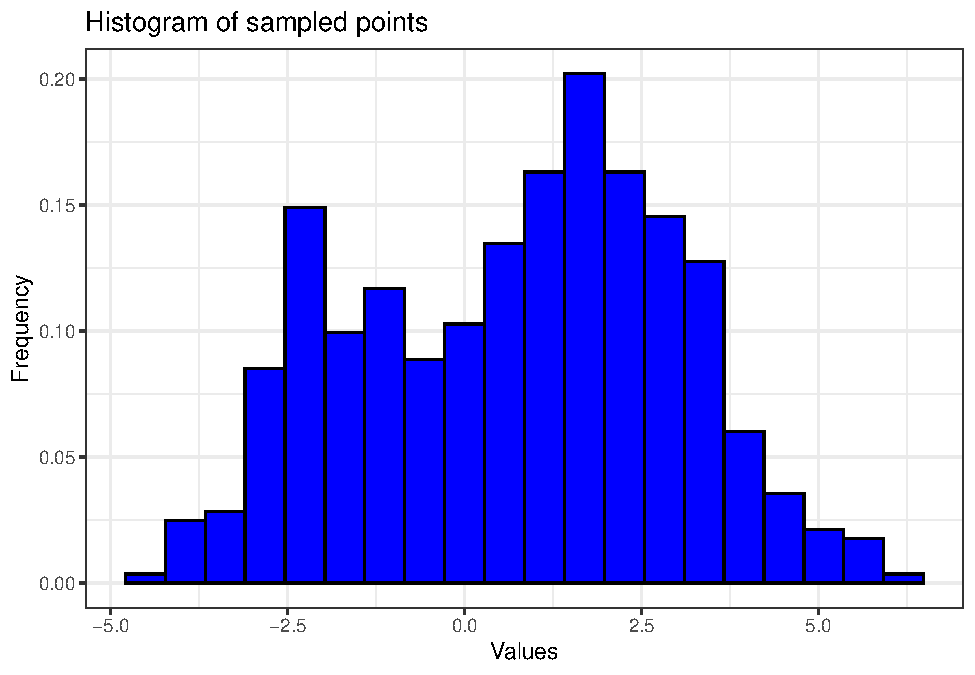
\includegraphics{direct_approach_kef_Brownian_kernel_files/figure-latex/unnamed-chunk-4-1.pdf}

\subsection{Find Gram Matrix of the sampled
points}\label{find-gram-matrix-of-the-sampled-points}

\begin{Shaded}
\begin{Highlighting}[]
\CommentTok{\# List of fixed points}
\NormalTok{list\_fixed\_points }\OtherTok{=} \FunctionTok{as.list}\NormalTok{(vec\_fixed\_points)}

\NormalTok{centering\_param }\OtherTok{\textless{}{-}} \DecValTok{7}
\CommentTok{\# Find the Gram matrix}
\NormalTok{gram }\OtherTok{\textless{}{-}} \FunctionTok{gram\_matrix}\NormalTok{(}\AttributeTok{vec\_list =}\NormalTok{ list\_fixed\_points, }
                    \AttributeTok{kernel\_type =} \StringTok{"uniform\_centered\_brownian"}\NormalTok{,}
                    \AttributeTok{kernel\_params =} \FunctionTok{list}\NormalTok{(}\AttributeTok{length\_scale =} \DecValTok{1}\NormalTok{, }\AttributeTok{degree =} \DecValTok{2}\NormalTok{,}
                                             \AttributeTok{free\_add =} \DecValTok{0}\NormalTok{, }\AttributeTok{free\_mult =} \DecValTok{1}\NormalTok{,}
                                             \AttributeTok{nu\_matern =} \DecValTok{1}\NormalTok{, }\AttributeTok{centering\_param =}\NormalTok{ centering\_param))}
\end{Highlighting}
\end{Shaded}

\subsection{True Kernel Mean
Embeddings}\label{true-kernel-mean-embeddings}

\begin{Shaded}
\begin{Highlighting}[]
\CommentTok{\# Grid of 100 points from {-}10 to 10}
\NormalTok{u }\OtherTok{\textless{}{-}}\NormalTok{ centering\_param}


\NormalTok{lambda }\OtherTok{\textless{}{-}} \DecValTok{1}

\CommentTok{\# Kernel mean embedding be careful change the mean if change the mean of P}


\CommentTok{\# Define the function f with point as a parameter}
\NormalTok{f }\OtherTok{\textless{}{-}} \ControlFlowTok{function}\NormalTok{(x, point, lambda, probabilities, means, sds, centering\_param) \{}
\NormalTok{  base\_measure\_gaussian\_mixture }\OtherTok{\textless{}{-}} \DecValTok{0}
  \ControlFlowTok{for}\NormalTok{ (i }\ControlFlowTok{in} \DecValTok{1}\SpecialCharTok{:}\FunctionTok{length}\NormalTok{(probabilities)) \{}
\NormalTok{    base\_measure\_gaussian\_mixture }\OtherTok{\textless{}{-}}\NormalTok{ base\_measure\_gaussian\_mixture }\SpecialCharTok{+}
\NormalTok{      probabilities[i] }\SpecialCharTok{/}\NormalTok{ (}\FunctionTok{sqrt}\NormalTok{(}\DecValTok{2} \SpecialCharTok{*}\NormalTok{ pi) }\SpecialCharTok{*}\NormalTok{ sds[i]) }\SpecialCharTok{*} \FunctionTok{exp}\NormalTok{(}\SpecialCharTok{{-}}\NormalTok{ (x }\SpecialCharTok{{-}}\NormalTok{ means[i])}\SpecialCharTok{\^{}}\DecValTok{2} \SpecialCharTok{/}\NormalTok{ (}\DecValTok{2} \SpecialCharTok{*}\NormalTok{ sds[i]}\SpecialCharTok{\^{}}\DecValTok{2}\NormalTok{)) }\SpecialCharTok{*}
      \FunctionTok{exp}\NormalTok{(}\SpecialCharTok{{-}}\NormalTok{lambda}\SpecialCharTok{/}\DecValTok{4}\SpecialCharTok{*}\NormalTok{(x}\SpecialCharTok{\^{}}\DecValTok{2}\SpecialCharTok{/}\NormalTok{centering\_param }\SpecialCharTok{+}\NormalTok{ centering\_param}\SpecialCharTok{/}\DecValTok{3}\NormalTok{))}
\NormalTok{  \}}

  \FunctionTok{return}\NormalTok{ ((lambda }\SpecialCharTok{/} \DecValTok{2}\NormalTok{) }\SpecialCharTok{*}\NormalTok{ (}\SpecialCharTok{{-}}\FunctionTok{abs}\NormalTok{(x }\SpecialCharTok{{-}}\NormalTok{ point) }\SpecialCharTok{+}\NormalTok{ (x}\SpecialCharTok{\^{}}\DecValTok{2} \SpecialCharTok{+}\NormalTok{ point}\SpecialCharTok{\^{}}\DecValTok{2}\NormalTok{) }\SpecialCharTok{/}\NormalTok{ (}\DecValTok{2} \SpecialCharTok{*}\NormalTok{ centering\_param) }\SpecialCharTok{+}\NormalTok{ centering\_param }\SpecialCharTok{/} \DecValTok{3}\NormalTok{) }\SpecialCharTok{*}\NormalTok{ base\_measure\_gaussian\_mixture)}
\NormalTok{\}}



\CommentTok{\# Define a wrapper function to perform integration}
\NormalTok{integrate\_for\_point }\OtherTok{\textless{}{-}} \ControlFlowTok{function}\NormalTok{(point, lambda, probabilities, means, sds, centering\_param) \{}
  \CommentTok{\# Calculate the integral part}
\NormalTok{  integral\_result }\OtherTok{\textless{}{-}} \FunctionTok{integrate}\NormalTok{(}\ControlFlowTok{function}\NormalTok{(x) }\FunctionTok{f}\NormalTok{(x, point, lambda, probabilities,}
\NormalTok{                                             means, sds, centering\_param),}
                               \AttributeTok{subdivisions =} \DecValTok{10000}\NormalTok{, }\AttributeTok{rel.tol =} \FloatTok{1e{-}10}\NormalTok{,}
                               \AttributeTok{abs.tol =} \FloatTok{1e{-}10}\NormalTok{,}\AttributeTok{lower =} \SpecialCharTok{{-}}\NormalTok{centering\_param, }\AttributeTok{upper =}\NormalTok{ centering\_param)}\SpecialCharTok{$}\NormalTok{value}

\NormalTok{  additional\_terms }\OtherTok{\textless{}{-}} \DecValTok{0}
  \ControlFlowTok{for}\NormalTok{ (i }\ControlFlowTok{in} \DecValTok{1}\SpecialCharTok{:}\FunctionTok{length}\NormalTok{(probabilities)) \{}
\NormalTok{    term1 }\OtherTok{\textless{}{-}}\NormalTok{ probabilities[i] }\SpecialCharTok{*}\NormalTok{ lambda }\SpecialCharTok{*}
\NormalTok{      (centering\_param}\SpecialCharTok{\^{}}\DecValTok{2} \SpecialCharTok{+} \DecValTok{6} \SpecialCharTok{*}\NormalTok{ centering\_param }\SpecialCharTok{*}\NormalTok{ point }\SpecialCharTok{{-}} \DecValTok{3} \SpecialCharTok{*}\NormalTok{ point}\SpecialCharTok{\^{}}\DecValTok{2}\NormalTok{) }\SpecialCharTok{*}
      \FunctionTok{exp}\NormalTok{(lambda}\SpecialCharTok{/}\DecValTok{24}\SpecialCharTok{*}\NormalTok{(}\DecValTok{12}\SpecialCharTok{*}\NormalTok{means[i]}\SpecialCharTok{+}\DecValTok{4}\SpecialCharTok{*}\NormalTok{centering\_param}\SpecialCharTok{+}\DecValTok{3}\SpecialCharTok{*}\NormalTok{sds[i]}\SpecialCharTok{\^{}}\DecValTok{2}\SpecialCharTok{*}\NormalTok{lambda))}\SpecialCharTok{/}\NormalTok{ (}\DecValTok{24} \SpecialCharTok{*}\NormalTok{ centering\_param)}
\NormalTok{    term2 }\OtherTok{\textless{}{-}}\NormalTok{ probabilities[i] }\SpecialCharTok{*}\NormalTok{ lambda }\SpecialCharTok{*}
\NormalTok{      (centering\_param}\SpecialCharTok{\^{}}\DecValTok{2} \SpecialCharTok{{-}} \DecValTok{6} \SpecialCharTok{*}\NormalTok{ centering\_param }\SpecialCharTok{*}\NormalTok{ point }\SpecialCharTok{{-}} \DecValTok{3} \SpecialCharTok{*}\NormalTok{ point}\SpecialCharTok{\^{}}\DecValTok{2}\NormalTok{) }\SpecialCharTok{*}
      \FunctionTok{exp}\NormalTok{(lambda}\SpecialCharTok{/}\DecValTok{24}\SpecialCharTok{*}\NormalTok{(}\SpecialCharTok{{-}}\DecValTok{12}\SpecialCharTok{*}\NormalTok{means[i]}\SpecialCharTok{+}\DecValTok{4}\SpecialCharTok{*}\NormalTok{centering\_param}\SpecialCharTok{+}\DecValTok{3}\SpecialCharTok{*}\NormalTok{sds[i]}\SpecialCharTok{\^{}}\DecValTok{2}\SpecialCharTok{*}\NormalTok{lambda))}\SpecialCharTok{/}\NormalTok{ (}\DecValTok{24} \SpecialCharTok{*}\NormalTok{ centering\_param)}
\NormalTok{    erf\_component1 }\OtherTok{\textless{}{-}} \FunctionTok{erfc}\NormalTok{((}\DecValTok{2}\SpecialCharTok{*}\NormalTok{(means[i] }\SpecialCharTok{+}\NormalTok{ centering\_param)}\SpecialCharTok{+}\NormalTok{ sds[i]}\SpecialCharTok{\^{}}\DecValTok{2}\SpecialCharTok{*}\NormalTok{lambda )}\SpecialCharTok{/}\NormalTok{ (}\DecValTok{2}\SpecialCharTok{*}\FunctionTok{sqrt}\NormalTok{(}\DecValTok{2}\NormalTok{) }\SpecialCharTok{*}\NormalTok{ sds[i]))}
\NormalTok{    erf\_component2 }\OtherTok{\textless{}{-}} \FunctionTok{erfc}\NormalTok{((}\DecValTok{2}\SpecialCharTok{*}\NormalTok{(}\SpecialCharTok{{-}}\NormalTok{means[i] }\SpecialCharTok{+}\NormalTok{ centering\_param)}\SpecialCharTok{+}\NormalTok{ sds[i]}\SpecialCharTok{\^{}}\DecValTok{2}\SpecialCharTok{*}\NormalTok{lambda )}\SpecialCharTok{/}\NormalTok{ (}\DecValTok{2}\SpecialCharTok{*}\FunctionTok{sqrt}\NormalTok{(}\DecValTok{2}\NormalTok{) }\SpecialCharTok{*}\NormalTok{ sds[i]))}

\NormalTok{    additional\_terms }\OtherTok{\textless{}{-}}\NormalTok{ additional\_terms }\SpecialCharTok{{-}}\NormalTok{ (term1 }\SpecialCharTok{*}\NormalTok{ erf\_component1) }\SpecialCharTok{{-}}\NormalTok{ (term2 }\SpecialCharTok{*}\NormalTok{ erf\_component2)}
\NormalTok{  \}}

\NormalTok{  result }\OtherTok{\textless{}{-}}\NormalTok{ integral\_result }\SpecialCharTok{+}\NormalTok{ additional\_terms}

  \FunctionTok{return}\NormalTok{(result)}
\NormalTok{\}}

\CommentTok{\# Apply the integration function to each element of grid\_point}
\NormalTok{KME\_true }\OtherTok{\textless{}{-}} \FunctionTok{sapply}\NormalTok{(vec\_fixed\_points, integrate\_for\_point,}
                   \AttributeTok{lambda =}\NormalTok{ lambda,}
                   \AttributeTok{probabilities =}\NormalTok{ probabilities,}
                   \AttributeTok{means =}\NormalTok{ means,}
                   \AttributeTok{sds =}\NormalTok{ sds,}
                   \AttributeTok{centering\_param =}\NormalTok{ centering\_param)}





\CommentTok{\# Data frame with true kernel mean embeddings}
\NormalTok{true\_KME }\OtherTok{\textless{}{-}} \FunctionTok{data.frame}\NormalTok{(vec\_fixed\_points, }\AttributeTok{true\_KME =}\NormalTok{ KME\_true)}
\end{Highlighting}
\end{Shaded}

\subsection{Kernel Mean Embedding Estimation: Standard
Estimator}\label{kernel-mean-embedding-estimation-standard-estimator}

\begin{Shaded}
\begin{Highlighting}[]
\CommentTok{\# Data frame with estimated kernel mean embedding}
\NormalTok{df\_std }\OtherTok{\textless{}{-}} \FunctionTok{data.frame}\NormalTok{(vec\_fixed\_points, }\AttributeTok{standard\_KME =} \FunctionTok{colMeans}\NormalTok{(gram))}

\CommentTok{\# Data frame for fixed points: adding e}
\NormalTok{df\_fixed\_points }\OtherTok{\textless{}{-}} \FunctionTok{data.frame}\NormalTok{(}\AttributeTok{x =}\NormalTok{ vec\_fixed\_points, }\AttributeTok{y =} \FunctionTok{rep}\NormalTok{(}\DecValTok{0}\NormalTok{, }\FunctionTok{length}\NormalTok{(vec\_fixed\_points)))}
\end{Highlighting}
\end{Shaded}

\subsubsection{Kernel Mean Embedding
Estimator}\label{kernel-mean-embedding-estimator}

\begin{Shaded}
\begin{Highlighting}[]
\CommentTok{\# Plot the results using ggplot}
\FunctionTok{library}\NormalTok{(ggplot2)}
\CommentTok{\# Create a combined data frame to handle both blue (standard) and orange (true KME) lines}
\NormalTok{df\_combined }\OtherTok{\textless{}{-}} \FunctionTok{rbind}\NormalTok{(}
  \FunctionTok{data.frame}\NormalTok{(}\AttributeTok{grid\_points =}\NormalTok{ df\_std}\SpecialCharTok{$}\NormalTok{vec\_fixed\_points, }\AttributeTok{value =}\NormalTok{ df\_std}\SpecialCharTok{$}\NormalTok{standard, }\AttributeTok{line =} \StringTok{"KME Estimator"}\NormalTok{),}
  \FunctionTok{data.frame}\NormalTok{(}\AttributeTok{grid\_points =}\NormalTok{ true\_KME}\SpecialCharTok{$}\NormalTok{vec\_fixed\_points, }\AttributeTok{value =}\NormalTok{ true\_KME}\SpecialCharTok{$}\NormalTok{true\_KME, }\AttributeTok{line =} \StringTok{"True KME"}\NormalTok{)}
\NormalTok{)}

\FunctionTok{ggplot}\NormalTok{() }\SpecialCharTok{+}
  \FunctionTok{geom\_hline}\NormalTok{(}\AttributeTok{yintercept =} \DecValTok{0}\NormalTok{, }\AttributeTok{color =} \StringTok{"gray"}\NormalTok{, }\AttributeTok{linetype =} \StringTok{"solid"}\NormalTok{, }\AttributeTok{linewidth =} \FloatTok{0.5}\NormalTok{) }\SpecialCharTok{+}  \CommentTok{\# Add axis y = 0}
  \FunctionTok{geom\_vline}\NormalTok{(}\AttributeTok{xintercept =} \DecValTok{0}\NormalTok{, }\AttributeTok{color =} \StringTok{"gray"}\NormalTok{, }\AttributeTok{linetype =} \StringTok{"solid"}\NormalTok{, }\AttributeTok{linewidth =} \FloatTok{0.5}\NormalTok{) }\SpecialCharTok{+}  \CommentTok{\# Add axis at x = 0}
  \FunctionTok{geom\_point}\NormalTok{(}\AttributeTok{data =}\NormalTok{ df\_fixed\_points, }\FunctionTok{aes}\NormalTok{(}\AttributeTok{x =}\NormalTok{ x, }\AttributeTok{y =}\NormalTok{ y), }\AttributeTok{color =} \StringTok{\textquotesingle{}red\textquotesingle{}}\NormalTok{, }\AttributeTok{size =} \DecValTok{2}\NormalTok{ ,}\AttributeTok{shape =}\DecValTok{3}\NormalTok{) }\SpecialCharTok{+}  \CommentTok{\# Plot x points with y = 0 in red}
  \FunctionTok{geom\_line}\NormalTok{(}\AttributeTok{data =}\NormalTok{ df\_combined, }\FunctionTok{aes}\NormalTok{(}\AttributeTok{x =}\NormalTok{ grid\_points, }\AttributeTok{y =}\NormalTok{ value, }\AttributeTok{color =}\NormalTok{ line), }\AttributeTok{linewidth =} \FloatTok{1.2}\NormalTok{) }\SpecialCharTok{+} \CommentTok{\# Plot both lines with color mapped to \textquotesingle{}line\textquotesingle{}}
  \FunctionTok{labs}\NormalTok{(}\AttributeTok{x =} \StringTok{"x"}\NormalTok{,}
       \AttributeTok{y =} \StringTok{"Standard Estimator $}\SpecialCharTok{\textbackslash{}\textbackslash{}}\StringTok{hat\{}\SpecialCharTok{\textbackslash{}\textbackslash{}}\StringTok{mu\}\_\{}\SpecialCharTok{\textbackslash{}\textbackslash{}}\StringTok{mathbb\{P\}\}"}\NormalTok{,}
       \AttributeTok{title =} \StringTok{"Standard Estimator of Kernel Mean Embedding"}\NormalTok{) }\SpecialCharTok{+}
  \FunctionTok{theme\_bw}\NormalTok{() }\SpecialCharTok{+}
  \FunctionTok{theme}\NormalTok{(}\AttributeTok{panel.grid =} \FunctionTok{element\_blank}\NormalTok{(),  }\CommentTok{\# Remove grid lines}
        \AttributeTok{panel.grid.major =} \FunctionTok{element\_blank}\NormalTok{(),}
        \AttributeTok{panel.grid.minor =} \FunctionTok{element\_blank}\NormalTok{()) }\SpecialCharTok{+}
  \FunctionTok{scale\_color\_manual}\NormalTok{(}\AttributeTok{values =} \FunctionTok{c}\NormalTok{(}\StringTok{"KME Estimator"} \OtherTok{=} \StringTok{"blue"}\NormalTok{, }\StringTok{"True KME"} \OtherTok{=} \StringTok{"orange"}\NormalTok{)) }\SpecialCharTok{+}  \CommentTok{\# Custom colors for the legend}
  \FunctionTok{guides}\NormalTok{(}\AttributeTok{color =} \FunctionTok{guide\_legend}\NormalTok{(}\AttributeTok{title =} \StringTok{"Type"}\NormalTok{))  }\CommentTok{\# Add a legend title}
\end{Highlighting}
\end{Shaded}

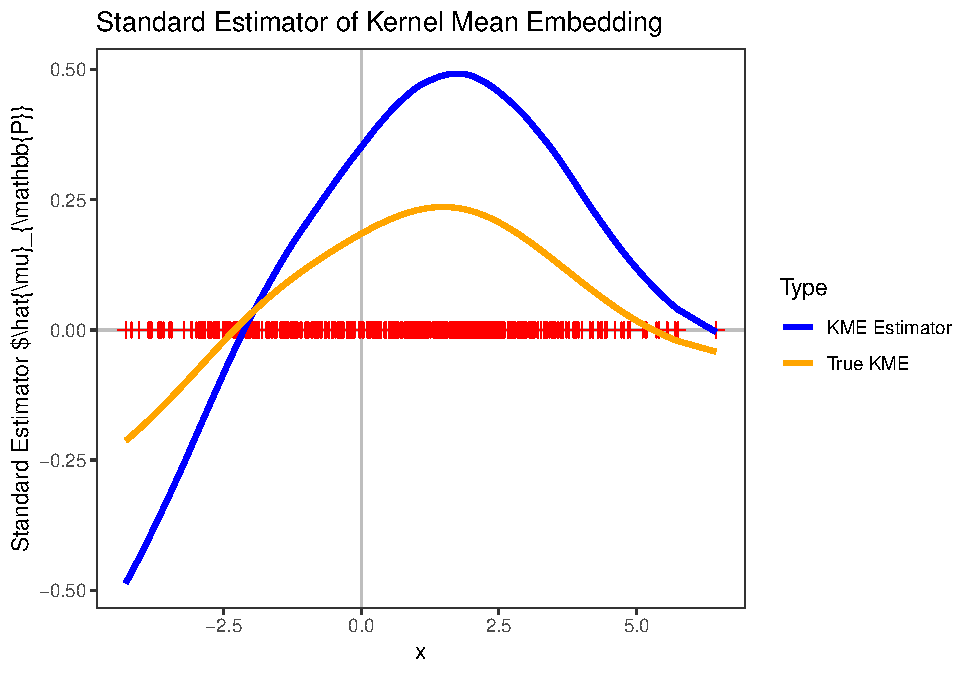
\includegraphics{direct_approach_kef_Brownian_kernel_files/figure-latex/unnamed-chunk-8-1.pdf}
\#\#\# Pre calculations:

\begin{Shaded}
\begin{Highlighting}[]
\CommentTok{\# Find the Gram matrix}
\NormalTok{gram }\OtherTok{\textless{}{-}} \FunctionTok{gram\_matrix}\NormalTok{(}\AttributeTok{vec\_list =}\NormalTok{ list\_fixed\_points, }
                    \AttributeTok{kernel\_type =} \StringTok{"uniform\_centered\_brownian"}\NormalTok{,}
                    \AttributeTok{kernel\_params =} \FunctionTok{list}\NormalTok{(}\AttributeTok{length\_scale =} \DecValTok{1}\NormalTok{, }\AttributeTok{degree =} \DecValTok{2}\NormalTok{,}
                                             \AttributeTok{free\_add =} \DecValTok{0}\NormalTok{, }\AttributeTok{free\_mult =} \DecValTok{1}\NormalTok{,}
                                             \AttributeTok{nu\_matern =} \DecValTok{1}\NormalTok{, }\AttributeTok{centering\_param =}\NormalTok{ centering\_param))}

\NormalTok{n }\OtherTok{=} \FunctionTok{length}\NormalTok{(list\_fixed\_points)}

\NormalTok{rho }\OtherTok{=} \DecValTok{1}\SpecialCharTok{/}\NormalTok{(n}\SpecialCharTok{\^{}}\DecValTok{2}\NormalTok{) }\SpecialCharTok{*} \FunctionTok{sum}\NormalTok{(gram)}

\NormalTok{rho\_with\_stroke }\OtherTok{=} \DecValTok{1}\SpecialCharTok{/}\NormalTok{n }\SpecialCharTok{*} \FunctionTok{sum}\NormalTok{(}\FunctionTok{diag}\NormalTok{(gram))}

\NormalTok{lambda\_reg }\OtherTok{=}\NormalTok{ n}\SpecialCharTok{*}\NormalTok{(rho\_with\_stroke}\SpecialCharTok{{-}}\NormalTok{rho) }\SpecialCharTok{/}\NormalTok{ ((n}\DecValTok{{-}1}\NormalTok{)}\SpecialCharTok{*}\NormalTok{(n}\SpecialCharTok{*}\NormalTok{rho}\SpecialCharTok{{-}}\NormalTok{rho\_with\_stroke))}
\end{Highlighting}
\end{Shaded}

\subsubsection{Find the shrinkage estimator of
KME:}\label{find-the-shrinkage-estimator-of-kme}

\begin{Shaded}
\begin{Highlighting}[]
\CommentTok{\# Function evaluation on the grid}
\NormalTok{results }\OtherTok{\textless{}{-}} \FunctionTok{sapply}\NormalTok{(vec\_fixed\_points, }\ControlFlowTok{function}\NormalTok{(point) \{}
  \FunctionTok{reg\_est\_KME}\NormalTok{(}\AttributeTok{evaluate\_at =}\NormalTok{ point,}
              \AttributeTok{list\_fixed =}\NormalTok{ list\_fixed\_points,}
              \AttributeTok{kernel\_type =} \StringTok{"uniform\_centered\_brownian"}\NormalTok{,}
              \AttributeTok{kernel\_params =} \FunctionTok{list}\NormalTok{(}\AttributeTok{length\_scale =} \DecValTok{1}\NormalTok{, }\AttributeTok{degree =} \DecValTok{2}\NormalTok{, }\AttributeTok{free\_add =} \DecValTok{0}\NormalTok{, }\AttributeTok{free\_mult =} \DecValTok{1}\NormalTok{, }\AttributeTok{nu\_matern =} \DecValTok{1}\NormalTok{, }\AttributeTok{centering\_param =}\NormalTok{ centering\_param),}
              \AttributeTok{precomputed =} \FunctionTok{list}\NormalTok{(}\AttributeTok{lambda =}\NormalTok{ lambda\_reg))}
\NormalTok{\})}


\CommentTok{\# Data frame with your data}
\NormalTok{df\_reg }\OtherTok{\textless{}{-}} \FunctionTok{data.frame}\NormalTok{(vec\_fixed\_points, }\AttributeTok{regularized =}\NormalTok{ results)}
\end{Highlighting}
\end{Shaded}

\subsection{Shrinkage Estimator of Kernel Mean Embedding
----}\label{shrinkage-estimator-of-kernel-mean-embedding--}

\subsubsection{Pre calculations:}\label{pre-calculations}

\begin{Shaded}
\begin{Highlighting}[]
\NormalTok{gram }\OtherTok{\textless{}{-}} \FunctionTok{gram\_matrix}\NormalTok{(}\AttributeTok{vec\_list =}\NormalTok{ list\_fixed\_points, }
                    \AttributeTok{kernel\_type =} \StringTok{"uniform\_centered\_brownian"}\NormalTok{,}
                    \AttributeTok{kernel\_params =} \FunctionTok{list}\NormalTok{(}\AttributeTok{length\_scale =} \DecValTok{1}\NormalTok{, }\AttributeTok{degree =} \DecValTok{2}\NormalTok{,}
                                             \AttributeTok{free\_add =} \DecValTok{0}\NormalTok{, }\AttributeTok{free\_mult =} \DecValTok{1}\NormalTok{,}
                                             \AttributeTok{nu\_matern =} \DecValTok{1}\NormalTok{, }
                                         \AttributeTok{centering\_param =}\NormalTok{ centering\_param))}

\NormalTok{n }\OtherTok{=} \FunctionTok{length}\NormalTok{(list\_fixed\_points)}

\NormalTok{lambda\_grid }\OtherTok{\textless{}{-}} \DecValTok{10}\SpecialCharTok{\^{}}\FunctionTok{seq}\NormalTok{(}\SpecialCharTok{{-}}\DecValTok{14}\NormalTok{,}\DecValTok{10}\NormalTok{,}\DecValTok{1}\NormalTok{)}

\NormalTok{lambda\_n\_grid }\OtherTok{\textless{}{-}} \DecValTok{10}\SpecialCharTok{\^{}}\FunctionTok{seq}\NormalTok{(}\SpecialCharTok{{-}}\DecValTok{14}\NormalTok{,}\DecValTok{10}\NormalTok{,}\DecValTok{1}\NormalTok{) }\SpecialCharTok{*}\NormalTok{ (n}\DecValTok{{-}1}\NormalTok{)}

\DocumentationTok{\#\#\# Precompute regularized inverses for each lambda\_n}

\NormalTok{regularized\_inverse\_grid }\OtherTok{\textless{}{-}} \FunctionTok{lapply}\NormalTok{(lambda\_n\_grid, }\ControlFlowTok{function}\NormalTok{(lambda\_n)\{}\FunctionTok{solve}\NormalTok{(gram }\SpecialCharTok{+}\NormalTok{ lambda\_n }\SpecialCharTok{*} \FunctionTok{diag}\NormalTok{(n))\})}
\end{Highlighting}
\end{Shaded}

\subsubsection{LOOCV hyper parameter
selection}\label{loocv-hyper-parameter-selection}

\begin{Shaded}
\begin{Highlighting}[]
\NormalTok{loocv\_values }\OtherTok{\textless{}{-}} \FunctionTok{rep}\NormalTok{(}\DecValTok{0}\NormalTok{,}\AttributeTok{length =} \FunctionTok{length}\NormalTok{(lambda\_grid))}
\DocumentationTok{\#\#\# Use sapply to iterate over lambda\_grid}
\NormalTok{loocv\_values }\OtherTok{\textless{}{-}} \FunctionTok{sapply}\NormalTok{(}\DecValTok{1}\SpecialCharTok{:}\FunctionTok{length}\NormalTok{(lambda\_grid), }\ControlFlowTok{function}\NormalTok{(i) \{}
  \FunctionTok{loocv\_shr}\NormalTok{(}\AttributeTok{gram =}\NormalTok{ gram, }\AttributeTok{lambda =}\NormalTok{ lambda\_grid[i], }\AttributeTok{precomp\_reg\_inv =}\NormalTok{ regularized\_inverse\_grid[[i]])}
\NormalTok{\})}
\end{Highlighting}
\end{Shaded}

\begin{verbatim}
## [1] "-"
## [1] "-"
## [1] "-"
## [1] "-"
## [1] "-"
## [1] "-"
## [1] "-"
## [1] "-"
## [1] "-"
## [1] "-"
## [1] "-"
## [1] "-"
## [1] "-"
## [1] "-"
## [1] "-"
## [1] "-"
## [1] "-"
## [1] "-"
## [1] "-"
## [1] "-"
## [1] "-"
## [1] "-"
## [1] "-"
## [1] "-"
## [1] "-"
\end{verbatim}

\begin{Shaded}
\begin{Highlighting}[]
\DocumentationTok{\#\#\# Create a dataframe to store lambda values and their corresponding LOOCV errors}
\NormalTok{loocv\_df }\OtherTok{\textless{}{-}} \FunctionTok{data.frame}\NormalTok{(}\AttributeTok{lambda =}\NormalTok{ lambda\_grid, }\AttributeTok{loocv =}\NormalTok{ loocv\_values)}

\DocumentationTok{\#\#\# Print the dataframe}
\FunctionTok{print}\NormalTok{(loocv\_df)}
\end{Highlighting}
\end{Shaded}

\begin{verbatim}
##    lambda    loocv
## 1   1e-14 1.310779
## 2   1e-13 1.292868
## 3   1e-12 1.292174
## 4   1e-11 1.292210
## 5   1e-10 1.292202
## 6   1e-09 1.292201
## 7   1e-08 1.292201
## 8   1e-07 1.292201
## 9   1e-06 1.292201
## 10  1e-05 1.292201
## 11  1e-04 1.292201
## 12  1e-03 1.292209
## 13  1e-02 1.292821
## 14  1e-01 1.308502
## 15  1e+00 1.429393
## 16  1e+01 1.543056
## 17  1e+02 1.563978
## 18  1e+03 1.566249
## 19  1e+04 1.566478
## 20  1e+05 1.566501
## 21  1e+06 1.566503
## 22  1e+07 1.566503
## 23  1e+08 1.566503
## 24  1e+09 1.566503
## 25  1e+10 1.566503
\end{verbatim}

\subsubsection{CV hyper parameter
selection}\label{cv-hyper-parameter-selection}

\begin{Shaded}
\begin{Highlighting}[]
\NormalTok{lambda\_grid }\OtherTok{\textless{}{-}} \FunctionTok{c}\NormalTok{(}\DecValTok{10}\SpecialCharTok{\^{}}\FunctionTok{seq}\NormalTok{(}\SpecialCharTok{{-}}\DecValTok{14}\NormalTok{,}\DecValTok{10}\NormalTok{,}\DecValTok{1}\NormalTok{))}

\NormalTok{cv\_values }\OtherTok{\textless{}{-}} \FunctionTok{rep}\NormalTok{(}\DecValTok{0}\NormalTok{,}\AttributeTok{length =} \FunctionTok{length}\NormalTok{(lambda\_grid))}
\DocumentationTok{\#\#\# Use sapply to iterate over lambda\_grid}
\NormalTok{cv\_values }\OtherTok{\textless{}{-}} \FunctionTok{sapply}\NormalTok{(}\DecValTok{1}\SpecialCharTok{:}\FunctionTok{length}\NormalTok{(lambda\_grid), }\ControlFlowTok{function}\NormalTok{(i) \{}
  \FunctionTok{cross\_validation}\NormalTok{(}\AttributeTok{gram =}\NormalTok{ gram, }\AttributeTok{lambda =}\NormalTok{ lambda\_grid[i], }\AttributeTok{folds\_number =} \FunctionTok{nrow}\NormalTok{(gram),}\AttributeTok{estimator\_type =} \StringTok{"shrinkage"}\NormalTok{)}
\NormalTok{\})}
\end{Highlighting}
\end{Shaded}

\begin{verbatim}
## [1] "-"
## [1] "-"
## [1] "-"
## [1] "-"
## [1] "-"
## [1] "-"
## [1] "-"
## [1] "-"
## [1] "-"
## [1] "-"
## [1] "-"
## [1] "-"
## [1] "-"
## [1] "-"
## [1] "-"
## [1] "-"
## [1] "-"
## [1] "-"
## [1] "-"
## [1] "-"
## [1] "-"
## [1] "-"
## [1] "-"
## [1] "-"
## [1] "-"
\end{verbatim}

\begin{Shaded}
\begin{Highlighting}[]
\DocumentationTok{\#\#\# Create a dataframe to store lambda values and their corresponding LOOCV errors}
\NormalTok{cv\_df }\OtherTok{\textless{}{-}} \FunctionTok{data.frame}\NormalTok{(}\AttributeTok{lambda =}\NormalTok{ lambda\_grid, }\AttributeTok{cv =}\NormalTok{ cv\_values)}

\DocumentationTok{\#\#\# Print the dataframe}
\FunctionTok{print}\NormalTok{(cv\_df)}
\end{Highlighting}
\end{Shaded}

\begin{verbatim}
##    lambda       cv
## 1   1e-14 1.292201
## 2   1e-13 1.292201
## 3   1e-12 1.292201
## 4   1e-11 1.292201
## 5   1e-10 1.292201
## 6   1e-09 1.292201
## 7   1e-08 1.292201
## 8   1e-07 1.292201
## 9   1e-06 1.292201
## 10  1e-05 1.292201
## 11  1e-04 1.292201
## 12  1e-03 1.292209
## 13  1e-02 1.292821
## 14  1e-01 1.308502
## 15  1e+00 1.429393
## 16  1e+01 1.543056
## 17  1e+02 1.563978
## 18  1e+03 1.566249
## 19  1e+04 1.566478
## 20  1e+05 1.566501
## 21  1e+06 1.566503
## 22  1e+07 1.566503
## 23  1e+08 1.566503
## 24  1e+09 1.566503
## 25  1e+10 1.566503
\end{verbatim}

\begin{Shaded}
\begin{Highlighting}[]
\FunctionTok{save.image}\NormalTok{(}\StringTok{"C:/Users/rouda/OneDrive/Research/Codes/R/kef/examples/rdata\_direct\_brownian\_3.RData"}\NormalTok{)}
\end{Highlighting}
\end{Shaded}

\subsubsection{Find the best hyper parameter and corresponding beta
weights}\label{find-the-best-hyper-parameter-and-corresponding-beta-weights}

\begin{Shaded}
\begin{Highlighting}[]
\NormalTok{merged\_num\_anal }\OtherTok{\textless{}{-}} \FunctionTok{merge}\NormalTok{(cv\_df,loocv\_df,}\AttributeTok{by =} \StringTok{"lambda"}\NormalTok{)}

\CommentTok{\# Choose the best lambda with lowest loocv}
\NormalTok{lambda\_shr }\OtherTok{\textless{}{-}}\NormalTok{ cv\_df[}\FunctionTok{which.min}\NormalTok{(cv\_df}\SpecialCharTok{$}\NormalTok{cv),}\StringTok{"lambda"}\NormalTok{]}

\CommentTok{\# Calculate inverse of regularizer}
\NormalTok{inverse\_regularizer }\OtherTok{\textless{}{-}} \FunctionTok{solve}\NormalTok{(gram }\SpecialCharTok{+}\NormalTok{ n }\SpecialCharTok{*}\NormalTok{ lambda\_shr}\SpecialCharTok{*}\FunctionTok{diag}\NormalTok{(n))}

\CommentTok{\# 1\_n vector}
\NormalTok{one\_n }\OtherTok{\textless{}{-}} \FunctionTok{rep}\NormalTok{(}\DecValTok{1}\NormalTok{,n)}\SpecialCharTok{/}\NormalTok{n}

\CommentTok{\# Find beta}
\NormalTok{beta\_s }\OtherTok{\textless{}{-}} \FunctionTok{sqrt}\NormalTok{(n) }\SpecialCharTok{*}\NormalTok{ inverse\_regularizer }\SpecialCharTok{\%*\%}\NormalTok{ gram }\SpecialCharTok{\%*\%}\NormalTok{  one\_n}
\end{Highlighting}
\end{Shaded}

\subsubsection{Find the shrinkage estimator of
KME}\label{find-the-shrinkage-estimator-of-kme-1}

\begin{Shaded}
\begin{Highlighting}[]
\CommentTok{\# Function evaluation on the grid}
\NormalTok{results }\OtherTok{\textless{}{-}} \FunctionTok{sapply}\NormalTok{(vec\_fixed\_points, }\ControlFlowTok{function}\NormalTok{(point) \{}
  \FunctionTok{shr\_est\_KME}\NormalTok{(}\AttributeTok{evaluate\_at =}\NormalTok{ point,}
              \AttributeTok{list\_fixed =}\NormalTok{ list\_fixed\_points,}
              \AttributeTok{lambda\_tunner =} \DecValTok{1}\NormalTok{,}
              \AttributeTok{kernel\_type =} \StringTok{"uniform\_centered\_brownian"}\NormalTok{,}
              \AttributeTok{kernel\_params =} \FunctionTok{list}\NormalTok{(}\AttributeTok{length\_scale =} \DecValTok{1}\NormalTok{, }\AttributeTok{degree =} \DecValTok{2}\NormalTok{, }\AttributeTok{free\_add =} \DecValTok{0}\NormalTok{, }\AttributeTok{free\_mult =} \DecValTok{1}\NormalTok{, }\AttributeTok{nu\_matern =} \DecValTok{1}\NormalTok{, }\AttributeTok{centering\_param =}\NormalTok{ centering\_param),}
              \AttributeTok{precomputed =} \FunctionTok{list}\NormalTok{(}\AttributeTok{beta\_s =}\NormalTok{ beta\_s))}
\NormalTok{\})}


\CommentTok{\# Data frame with your data}
\NormalTok{df\_shr }\OtherTok{\textless{}{-}} \FunctionTok{data.frame}\NormalTok{(vec\_fixed\_points, }\AttributeTok{shrinkage =}\NormalTok{ results)}
\end{Highlighting}
\end{Shaded}

\subsection{Merge all the KME estimators and
plot}\label{merge-all-the-kme-estimators-and-plot}

\begin{Shaded}
\begin{Highlighting}[]
\NormalTok{df\_all }\OtherTok{\textless{}{-}} \FunctionTok{merge}\NormalTok{(df\_std,df\_reg,}\AttributeTok{by =} \StringTok{"vec\_fixed\_points"}\NormalTok{)}
\NormalTok{df\_all }\OtherTok{\textless{}{-}} \FunctionTok{merge}\NormalTok{(df\_all,df\_shr,}\AttributeTok{by =} \StringTok{"vec\_fixed\_points"}\NormalTok{)}
\NormalTok{df\_all }\OtherTok{\textless{}{-}} \FunctionTok{merge}\NormalTok{(df\_all,true\_KME,}\AttributeTok{by =} \StringTok{"vec\_fixed\_points"}\NormalTok{)}

\FunctionTok{save.image}\NormalTok{(}\StringTok{"C:/Users/rouda/OneDrive/Research/Codes/R/kef/examples/rdata\_direct\_4.RData"}\NormalTok{)}
\end{Highlighting}
\end{Shaded}

\begin{Shaded}
\begin{Highlighting}[]
\FunctionTok{load}\NormalTok{(}\StringTok{"C:/Users/rouda/OneDrive/Research/Codes/R/kef/examples/rdata\_direct\_4.RData"}\NormalTok{)}
\end{Highlighting}
\end{Shaded}

\begin{Shaded}
\begin{Highlighting}[]
\FunctionTok{library}\NormalTok{(tidyr)}

\CommentTok{\#gather data from columns 2 and 3}
\NormalTok{df\_long }\OtherTok{\textless{}{-}} \FunctionTok{gather}\NormalTok{(df\_all, }\AttributeTok{key=}\StringTok{"type"}\NormalTok{, }\AttributeTok{value=}\StringTok{"estimation"}\NormalTok{, }\DecValTok{2}\SpecialCharTok{:}\DecValTok{5}\NormalTok{)}

\NormalTok{df\_long}\SpecialCharTok{$}\NormalTok{type }\OtherTok{\textless{}{-}} \FunctionTok{factor}\NormalTok{(df\_long}\SpecialCharTok{$}\NormalTok{type, }\AttributeTok{levels =} \FunctionTok{colnames}\NormalTok{(df\_all)[}\SpecialCharTok{{-}}\DecValTok{1}\NormalTok{])}

\CommentTok{\# Data frame for fixed points:}
\NormalTok{df\_fixed\_points }\OtherTok{\textless{}{-}} \FunctionTok{data.frame}\NormalTok{(}\AttributeTok{x =}\NormalTok{ vec\_fixed\_points, }\AttributeTok{y =} \FunctionTok{rep}\NormalTok{(}\DecValTok{0}\NormalTok{, }\FunctionTok{length}\NormalTok{(vec\_fixed\_points)))}
\end{Highlighting}
\end{Shaded}

\begin{Shaded}
\begin{Highlighting}[]
\CommentTok{\# Plot the results using ggplot}
\FunctionTok{library}\NormalTok{(ggplot2)}
\FunctionTok{ggplot}\NormalTok{(df\_long, }\FunctionTok{aes}\NormalTok{(}\AttributeTok{x =}\NormalTok{ vec\_fixed\_points, }\AttributeTok{y =}\NormalTok{ estimation, }\AttributeTok{color =}\NormalTok{ type)) }\SpecialCharTok{+}
  \FunctionTok{geom\_hline}\NormalTok{(}\AttributeTok{yintercept =} \DecValTok{0}\NormalTok{, }\AttributeTok{color =} \StringTok{"gray"}\NormalTok{, }\AttributeTok{linetype =} \StringTok{"solid"}\NormalTok{, }\AttributeTok{linewidth =} \FloatTok{0.5}\NormalTok{) }\SpecialCharTok{+}  \CommentTok{\# Add axis y = 0}
  \FunctionTok{geom\_vline}\NormalTok{(}\AttributeTok{xintercept =} \DecValTok{0}\NormalTok{, }\AttributeTok{color =} \StringTok{"gray"}\NormalTok{, }\AttributeTok{linetype =} \StringTok{"solid"}\NormalTok{, }\AttributeTok{linewidth =} \FloatTok{0.5}\NormalTok{) }\SpecialCharTok{+}  \CommentTok{\# Add axis at x = 0}
  \FunctionTok{geom\_point}\NormalTok{(}\AttributeTok{data =}\NormalTok{ df\_fixed\_points, }\FunctionTok{aes}\NormalTok{(}\AttributeTok{x =}\NormalTok{ x, }\AttributeTok{y =}\NormalTok{ y), }\AttributeTok{color =} \StringTok{\textquotesingle{}red\textquotesingle{}}\NormalTok{, }\AttributeTok{size =} \DecValTok{2}\NormalTok{ ,}\AttributeTok{shape =}\DecValTok{3}\NormalTok{) }\SpecialCharTok{+}  \CommentTok{\# Plot x points with y = 0 in red}
  \FunctionTok{geom\_line}\NormalTok{(}\AttributeTok{linewidth =} \FloatTok{1.2}\NormalTok{) }\SpecialCharTok{+} \CommentTok{\# Plot kernel mean embedding estimator}
  \FunctionTok{labs}\NormalTok{(}\AttributeTok{x =} \StringTok{"x"}\NormalTok{,}
       \AttributeTok{y =} \StringTok{"Estimator $}\SpecialCharTok{\textbackslash{}\textbackslash{}}\StringTok{hat\{}\SpecialCharTok{\textbackslash{}\textbackslash{}}\StringTok{mu\}\_\{}\SpecialCharTok{\textbackslash{}\textbackslash{}}\StringTok{mathbb\{P\}\}(x)"}\NormalTok{,}
       \AttributeTok{title =} \StringTok{"Estimator of Kernel Mean Embedding"}\NormalTok{)}\SpecialCharTok{+}
  \FunctionTok{theme\_bw}\NormalTok{()}\SpecialCharTok{+}
  \FunctionTok{theme}\NormalTok{(}\AttributeTok{panel.grid =} \FunctionTok{element\_blank}\NormalTok{(),  }\CommentTok{\# Remove grid lines}
        \AttributeTok{panel.grid.major =} \FunctionTok{element\_blank}\NormalTok{(),}
        \AttributeTok{panel.grid.minor =} \FunctionTok{element\_blank}\NormalTok{()) }\SpecialCharTok{+}  \CommentTok{\# Axis ticks color}
  \FunctionTok{scale\_color\_manual}\NormalTok{(}\AttributeTok{values =} \FunctionTok{c}\NormalTok{(}\StringTok{\textquotesingle{}orange\textquotesingle{}}\NormalTok{, }\StringTok{\textquotesingle{}green\textquotesingle{}}\NormalTok{, }\StringTok{\textquotesingle{}green3\textquotesingle{}}\NormalTok{, }\StringTok{\textquotesingle{}blue\textquotesingle{}}\NormalTok{)) }\CommentTok{\# Customize colors}
\end{Highlighting}
\end{Shaded}

\includegraphics{direct_approach_kef_Brownian_kernel_files/figure-latex/unnamed-chunk-19-1.pdf}

\begin{Shaded}
\begin{Highlighting}[]
\FunctionTok{library}\NormalTok{(dplyr)}
\end{Highlighting}
\end{Shaded}

\begin{verbatim}
## 
## Attaching package: 'dplyr'
\end{verbatim}

\begin{verbatim}
## The following objects are masked from 'package:stats':
## 
##     filter, lag
\end{verbatim}

\begin{verbatim}
## The following objects are masked from 'package:base':
## 
##     intersect, setdiff, setequal, union
\end{verbatim}

\begin{Shaded}
\begin{Highlighting}[]
\CommentTok{\# Plot the results using ggplot}
\FunctionTok{ggplot}\NormalTok{(df\_long }\SpecialCharTok{\%\textgreater{}\%} \FunctionTok{filter}\NormalTok{(type }\SpecialCharTok{\%in\%} \FunctionTok{c}\NormalTok{(}\StringTok{"standard\_KME"}\NormalTok{,}\StringTok{"true\_KME"}\NormalTok{)), }\FunctionTok{aes}\NormalTok{(}\AttributeTok{x =}\NormalTok{ vec\_fixed\_points, }\AttributeTok{y =}\NormalTok{ estimation, }\AttributeTok{color =}\NormalTok{ type)) }\SpecialCharTok{+}
  \FunctionTok{geom\_hline}\NormalTok{(}\AttributeTok{yintercept =} \DecValTok{0}\NormalTok{, }\AttributeTok{color =} \StringTok{"gray"}\NormalTok{, }\AttributeTok{linetype =} \StringTok{"solid"}\NormalTok{, }\AttributeTok{linewidth =} \FloatTok{0.5}\NormalTok{) }\SpecialCharTok{+}  \CommentTok{\# Add axis y = 0}
  \FunctionTok{geom\_vline}\NormalTok{(}\AttributeTok{xintercept =} \DecValTok{0}\NormalTok{, }\AttributeTok{color =} \StringTok{"gray"}\NormalTok{, }\AttributeTok{linetype =} \StringTok{"solid"}\NormalTok{, }\AttributeTok{linewidth =} \FloatTok{0.5}\NormalTok{) }\SpecialCharTok{+}  \CommentTok{\# Add axis at x = 0}
  \FunctionTok{geom\_point}\NormalTok{(}\AttributeTok{data =}\NormalTok{ df\_fixed\_points, }\FunctionTok{aes}\NormalTok{(}\AttributeTok{x =}\NormalTok{ x, }\AttributeTok{y =}\NormalTok{ y), }\AttributeTok{color =} \StringTok{\textquotesingle{}red\textquotesingle{}}\NormalTok{, }\AttributeTok{size =} \DecValTok{2}\NormalTok{ ,}\AttributeTok{shape =}\DecValTok{3}\NormalTok{) }\SpecialCharTok{+}  \CommentTok{\# Plot x points with y = 0 in red}
  \FunctionTok{geom\_line}\NormalTok{(}\AttributeTok{linewidth =} \FloatTok{1.2}\NormalTok{) }\SpecialCharTok{+} \CommentTok{\# Plot kernel mean embedding estimator}
  \FunctionTok{labs}\NormalTok{(}\AttributeTok{x =} \StringTok{"x"}\NormalTok{,}
       \AttributeTok{y =} \StringTok{"Estimator $}\SpecialCharTok{\textbackslash{}\textbackslash{}}\StringTok{hat\{}\SpecialCharTok{\textbackslash{}\textbackslash{}}\StringTok{mu\}\_\{P\}(x)$"}\NormalTok{,}
       \AttributeTok{title =} \StringTok{"Estimator of Kernel Mean Embedding"}\NormalTok{)}\SpecialCharTok{+}
  \FunctionTok{theme\_bw}\NormalTok{()}\SpecialCharTok{+}
  \FunctionTok{theme}\NormalTok{(}\AttributeTok{panel.grid =} \FunctionTok{element\_blank}\NormalTok{(),  }\CommentTok{\# Remove grid lines}
        \AttributeTok{panel.grid.major =} \FunctionTok{element\_blank}\NormalTok{(),}
        \AttributeTok{panel.grid.minor =} \FunctionTok{element\_blank}\NormalTok{()) }\SpecialCharTok{+}  \CommentTok{\# Axis ticks color}
  \FunctionTok{scale\_color\_manual}\NormalTok{(}\AttributeTok{values =} \FunctionTok{c}\NormalTok{(}\StringTok{\textquotesingle{}orange\textquotesingle{}}\NormalTok{,}\StringTok{\textquotesingle{}blue\textquotesingle{}}\NormalTok{)) }\CommentTok{\# Customize colors}
\end{Highlighting}
\end{Shaded}

\includegraphics{direct_approach_kef_Brownian_kernel_files/figure-latex/unnamed-chunk-20-1.pdf}

\begin{Shaded}
\begin{Highlighting}[]
\CommentTok{\# Plot the results using ggplot}
\FunctionTok{ggplot}\NormalTok{(df\_long }\SpecialCharTok{\%\textgreater{}\%} \FunctionTok{filter}\NormalTok{(type }\SpecialCharTok{\%in\%} \FunctionTok{c}\NormalTok{(}\StringTok{"regularized"}\NormalTok{,}\StringTok{"true\_KME"}\NormalTok{)), }\FunctionTok{aes}\NormalTok{(}\AttributeTok{x =}\NormalTok{ vec\_fixed\_points, }\AttributeTok{y =}\NormalTok{ estimation, }\AttributeTok{color =}\NormalTok{ type)) }\SpecialCharTok{+}
  \FunctionTok{geom\_hline}\NormalTok{(}\AttributeTok{yintercept =} \DecValTok{0}\NormalTok{, }\AttributeTok{color =} \StringTok{"gray"}\NormalTok{, }\AttributeTok{linetype =} \StringTok{"solid"}\NormalTok{, }\AttributeTok{linewidth =} \FloatTok{0.5}\NormalTok{) }\SpecialCharTok{+}  \CommentTok{\# Add axis y = 0}
  \FunctionTok{geom\_vline}\NormalTok{(}\AttributeTok{xintercept =} \DecValTok{0}\NormalTok{, }\AttributeTok{color =} \StringTok{"gray"}\NormalTok{, }\AttributeTok{linetype =} \StringTok{"solid"}\NormalTok{, }\AttributeTok{linewidth =} \FloatTok{0.5}\NormalTok{) }\SpecialCharTok{+}  \CommentTok{\# Add axis at x = 0}
  \FunctionTok{geom\_point}\NormalTok{(}\AttributeTok{data =}\NormalTok{ df\_fixed\_points, }\FunctionTok{aes}\NormalTok{(}\AttributeTok{x =}\NormalTok{ x, }\AttributeTok{y =}\NormalTok{ y), }\AttributeTok{color =} \StringTok{\textquotesingle{}red\textquotesingle{}}\NormalTok{, }\AttributeTok{size =} \DecValTok{2}\NormalTok{ ,}\AttributeTok{shape =}\DecValTok{3}\NormalTok{) }\SpecialCharTok{+}  \CommentTok{\# Plot x points with y = 0 in red}
  \FunctionTok{geom\_line}\NormalTok{(}\AttributeTok{linewidth =} \FloatTok{1.2}\NormalTok{) }\SpecialCharTok{+} \CommentTok{\# Plot kernel mean embedding estimator}
  \FunctionTok{labs}\NormalTok{(}\AttributeTok{x =} \StringTok{"x"}\NormalTok{,}
       \AttributeTok{y =} \StringTok{"Estimator $}\SpecialCharTok{\textbackslash{}\textbackslash{}}\StringTok{hat\{}\SpecialCharTok{\textbackslash{}\textbackslash{}}\StringTok{mu\}\_\{}\SpecialCharTok{\textbackslash{}\textbackslash{}}\StringTok{mathbb\{P\}\}(x)"}\NormalTok{,}
       \AttributeTok{title =} \StringTok{"Estimator of Kernel Mean Embedding"}\NormalTok{)}\SpecialCharTok{+}
  \FunctionTok{theme\_bw}\NormalTok{()}\SpecialCharTok{+}
  \FunctionTok{theme}\NormalTok{(}\AttributeTok{panel.grid =} \FunctionTok{element\_blank}\NormalTok{(),  }\CommentTok{\# Remove grid lines}
        \AttributeTok{panel.grid.major =} \FunctionTok{element\_blank}\NormalTok{(),}
        \AttributeTok{panel.grid.minor =} \FunctionTok{element\_blank}\NormalTok{()) }\SpecialCharTok{+}  \CommentTok{\# Axis ticks color}
  \FunctionTok{scale\_color\_manual}\NormalTok{(}\AttributeTok{values =} \FunctionTok{c}\NormalTok{(}\StringTok{\textquotesingle{}green\textquotesingle{}}\NormalTok{,}\StringTok{\textquotesingle{}blue\textquotesingle{}}\NormalTok{)) }\CommentTok{\# Customize colors}
\end{Highlighting}
\end{Shaded}

\includegraphics{direct_approach_kef_Brownian_kernel_files/figure-latex/unnamed-chunk-21-1.pdf}

\begin{Shaded}
\begin{Highlighting}[]
\CommentTok{\# Plot the results using ggplot}
\FunctionTok{ggplot}\NormalTok{(df\_long }\SpecialCharTok{\%\textgreater{}\%} \FunctionTok{filter}\NormalTok{(type }\SpecialCharTok{\%in\%} \FunctionTok{c}\NormalTok{(}\StringTok{"shrinkage"}\NormalTok{,}\StringTok{"true\_KME"}\NormalTok{)), }\FunctionTok{aes}\NormalTok{(}\AttributeTok{x =}\NormalTok{ vec\_fixed\_points, }\AttributeTok{y =}\NormalTok{ estimation, }\AttributeTok{color =}\NormalTok{ type)) }\SpecialCharTok{+}
  \FunctionTok{geom\_hline}\NormalTok{(}\AttributeTok{yintercept =} \DecValTok{0}\NormalTok{, }\AttributeTok{color =} \StringTok{"gray"}\NormalTok{, }\AttributeTok{linetype =} \StringTok{"solid"}\NormalTok{, }\AttributeTok{linewidth =} \FloatTok{0.5}\NormalTok{) }\SpecialCharTok{+}  \CommentTok{\# Add axis y = 0}
  \FunctionTok{geom\_vline}\NormalTok{(}\AttributeTok{xintercept =} \DecValTok{0}\NormalTok{, }\AttributeTok{color =} \StringTok{"gray"}\NormalTok{, }\AttributeTok{linetype =} \StringTok{"solid"}\NormalTok{, }\AttributeTok{linewidth =} \FloatTok{0.5}\NormalTok{) }\SpecialCharTok{+}  \CommentTok{\# Add axis at x = 0}
  \FunctionTok{geom\_point}\NormalTok{(}\AttributeTok{data =}\NormalTok{ df\_fixed\_points, }\FunctionTok{aes}\NormalTok{(}\AttributeTok{x =}\NormalTok{ x, }\AttributeTok{y =}\NormalTok{ y), }\AttributeTok{color =} \StringTok{\textquotesingle{}red\textquotesingle{}}\NormalTok{, }\AttributeTok{size =} \DecValTok{2}\NormalTok{ ,}\AttributeTok{shape =}\DecValTok{3}\NormalTok{) }\SpecialCharTok{+}  \CommentTok{\# Plot x points with y = 0 in red}
  \FunctionTok{geom\_line}\NormalTok{(}\AttributeTok{linewidth =} \FloatTok{1.2}\NormalTok{) }\SpecialCharTok{+} \CommentTok{\# Plot kernel mean embedding estimator}
  \FunctionTok{labs}\NormalTok{(}\AttributeTok{x =} \StringTok{"x"}\NormalTok{,}
       \AttributeTok{y =} \StringTok{"Estimator $}\SpecialCharTok{\textbackslash{}\textbackslash{}}\StringTok{hat\{}\SpecialCharTok{\textbackslash{}\textbackslash{}}\StringTok{mu\}\_\{}\SpecialCharTok{\textbackslash{}\textbackslash{}}\StringTok{mathbb\{P\}\}(x)"}\NormalTok{,}
       \AttributeTok{title =} \StringTok{"Estimator of Kernel Mean Embedding"}\NormalTok{)}\SpecialCharTok{+}
  \FunctionTok{theme\_bw}\NormalTok{()}\SpecialCharTok{+}
  \FunctionTok{theme}\NormalTok{(}\AttributeTok{panel.grid =} \FunctionTok{element\_blank}\NormalTok{(),  }\CommentTok{\# Remove grid lines}
        \AttributeTok{panel.grid.major =} \FunctionTok{element\_blank}\NormalTok{(),}
        \AttributeTok{panel.grid.minor =} \FunctionTok{element\_blank}\NormalTok{()) }\SpecialCharTok{+}  \CommentTok{\# Axis ticks color}
  \FunctionTok{scale\_color\_manual}\NormalTok{(}\AttributeTok{values =} \FunctionTok{c}\NormalTok{(}\StringTok{\textquotesingle{}green3\textquotesingle{}}\NormalTok{,}\StringTok{\textquotesingle{}blue\textquotesingle{}}\NormalTok{)) }\CommentTok{\# Customize colors}
\end{Highlighting}
\end{Shaded}

\includegraphics{direct_approach_kef_Brownian_kernel_files/figure-latex/unnamed-chunk-22-1.pdf}

\section{Find the probabilities using KME and centered
kernel}\label{find-the-probabilities-using-kme-and-centered-kernel}

The relationship for \(\hat{\mu}(\mathbf{x}_i)\) is given by: \[
    \hat{\mu}(\mathbf{x}_i) = \sum_{j=1}^n h(\mathbf{x}_i, \mathbf{x}_j) p_\theta(\mathbf{x}_j).
\] Furthermore, we can estimate \(\hat{\mu}(\mathbf{x}_i)\) using
methods like shrinkage or Bayesian approaches: Moreover, we can estimate
\(\hat{\mu}(\mathbf{x}_i)\) with methods like shrinkage methods
\citep{muandet2016kernelmeanshrinkageestimators} and Bayesian method
\citep{flaxman2016bayesianlearningkernelembeddings}. So we can say
\(\hat{\mathbf{p}}_\theta = \mathbf{H}_{sample}^{-1} \hat{\boldsymbol{\mu}}\)

This allows us to form equations where only \(\theta\)'s are unknown: So
we can make equations that only \(\theta\)'s are unknown, and we can
find these parameters using estimated kernel mean embeddings.

Recall that the relationship for \(p_\theta(\mathbf{x}_j)\) is: \[
    \hat{p}_\theta(\mathbf{x}_j) = \dfrac{\exp(\hat{\theta}_n(\mathbf{x}_j))}{\sum_{j =1}^n \exp(\hat{\theta}_n(\mathbf{x}_j))}.
\]

\subsection{Specify the grid and centering
grid}\label{specify-the-grid-and-centering-grid}

\begin{Shaded}
\begin{Highlighting}[]
\NormalTok{sampled\_x }\OtherTok{\textless{}{-}}\NormalTok{ vec\_fixed\_points}
\NormalTok{x\_grid }\OtherTok{\textless{}{-}}  \FunctionTok{seq}\NormalTok{(}\SpecialCharTok{{-}}\DecValTok{7}\NormalTok{,}\DecValTok{7}\NormalTok{,}\AttributeTok{length.out =} \DecValTok{1000}\NormalTok{)}
\CommentTok{\# centering\_grid \textless{}{-} sampled\_x This doesn\textquotesingle{}t work because using this centering grid the kernel mean embedding is zero.}
\NormalTok{centering\_grid }\OtherTok{\textless{}{-}} \FunctionTok{runif}\NormalTok{(}\AttributeTok{min =} \SpecialCharTok{{-}}\DecValTok{7}\NormalTok{,}\AttributeTok{max =} \DecValTok{7}\NormalTok{,}\AttributeTok{n =} \DecValTok{1000}\NormalTok{)}
\end{Highlighting}
\end{Shaded}

\subsection{Find Kernel Matrices:}\label{find-kernel-matrices}

\(\mathbf{H}_{sample}\):

\begin{Shaded}
\begin{Highlighting}[]
\NormalTok{centered\_kernel\_mat\_at\_sampled }\OtherTok{\textless{}{-}} \FunctionTok{centered\_kernel\_matrix}\NormalTok{(}\AttributeTok{first\_vec\_kernel =}\NormalTok{ sampled\_x,}
                                                         \AttributeTok{second\_vec\_kernel =}\NormalTok{ sampled\_x,}
                                                         \AttributeTok{centering\_grid =}\NormalTok{ centering\_grid,}
                                                         \AttributeTok{hurst\_coef =} \FloatTok{0.5}\NormalTok{)}
\end{Highlighting}
\end{Shaded}

\begin{Shaded}
\begin{Highlighting}[]
\FunctionTok{library}\NormalTok{(ggplot2)}
\FunctionTok{library}\NormalTok{(reshape2)}
\end{Highlighting}
\end{Shaded}

\begin{verbatim}
## Warning: package 'reshape2' was built under R version 4.3.2
\end{verbatim}

\begin{verbatim}
## 
## Attaching package: 'reshape2'
\end{verbatim}

\begin{verbatim}
## The following object is masked from 'package:tidyr':
## 
##     smiths
\end{verbatim}

\begin{Shaded}
\begin{Highlighting}[]
\CommentTok{\# Convert matrix to a data frame}
\NormalTok{matrix\_df }\OtherTok{\textless{}{-}} \FunctionTok{melt}\NormalTok{(centered\_kernel\_mat\_at\_sampled)}

\CommentTok{\# Plot using ggplot2}
\FunctionTok{ggplot}\NormalTok{(matrix\_df, }\FunctionTok{aes}\NormalTok{(Var1, Var2, }\AttributeTok{fill =}\NormalTok{ value)) }\SpecialCharTok{+}
  \FunctionTok{geom\_tile}\NormalTok{() }\SpecialCharTok{+}
  \FunctionTok{scale\_fill\_gradient2}\NormalTok{(}\AttributeTok{low =} \StringTok{"blue"}\NormalTok{, }\AttributeTok{mid =} \StringTok{"white"}\NormalTok{, }\AttributeTok{high =} \StringTok{"red"}\NormalTok{) }\SpecialCharTok{+}
  \FunctionTok{theme\_minimal}\NormalTok{() }\SpecialCharTok{+}
  \FunctionTok{coord\_fixed}\NormalTok{() }\SpecialCharTok{+}  \CommentTok{\# Ensures the plot is square}
  \FunctionTok{labs}\NormalTok{(}\AttributeTok{title =} \StringTok{"Centered Brownian Kernel wrt to uniform samples from {-}7 to 7"}\NormalTok{, }\AttributeTok{x =} \StringTok{"Sampled x"}\NormalTok{, }\AttributeTok{y =} \StringTok{"Sampled x"}\NormalTok{)}
\end{Highlighting}
\end{Shaded}

\includegraphics{direct_approach_kef_Brownian_kernel_files/figure-latex/unnamed-chunk-25-1.pdf}

\begin{Shaded}
\begin{Highlighting}[]
\CommentTok{\# Convert matrix to a data frame}
\NormalTok{matrix\_df }\OtherTok{\textless{}{-}} \FunctionTok{melt}\NormalTok{(gram)}

\CommentTok{\# Plot using ggplot2}
\FunctionTok{ggplot}\NormalTok{(matrix\_df, }\FunctionTok{aes}\NormalTok{(Var1, Var2, }\AttributeTok{fill =}\NormalTok{ value)) }\SpecialCharTok{+}
  \FunctionTok{geom\_tile}\NormalTok{() }\SpecialCharTok{+}
  \FunctionTok{scale\_fill\_gradient2}\NormalTok{(}\AttributeTok{low =} \StringTok{"blue"}\NormalTok{, }\AttributeTok{mid =} \StringTok{"white"}\NormalTok{, }\AttributeTok{high =} \StringTok{"red"}\NormalTok{) }\SpecialCharTok{+}
  \FunctionTok{theme\_minimal}\NormalTok{() }\SpecialCharTok{+}
  \FunctionTok{coord\_fixed}\NormalTok{() }\SpecialCharTok{+}  \CommentTok{\# Ensures the plot is square}
  \FunctionTok{labs}\NormalTok{(}\AttributeTok{title =} \StringTok{"Initial gram matrix centered wrt a uniform distribution from {-}7 to 7"}\NormalTok{, }\AttributeTok{x =} \StringTok{"Sampled x"}\NormalTok{, }\AttributeTok{y =} \StringTok{"Sampled x"}\NormalTok{)}
\end{Highlighting}
\end{Shaded}

\includegraphics{direct_approach_kef_Brownian_kernel_files/figure-latex/unnamed-chunk-26-1.pdf}

\begin{Shaded}
\begin{Highlighting}[]
\CommentTok{\# Positive Definiteness of centered\_kernel\_mat\_at\_sampled}

\CommentTok{\# Get the eigenvalues}
\NormalTok{eigenvalues }\OtherTok{\textless{}{-}} \FunctionTok{eigen}\NormalTok{(centered\_kernel\_mat\_at\_sampled)}\SpecialCharTok{$}\NormalTok{values}

\CommentTok{\# Check if all eigenvalues are positive}
\NormalTok{is\_positive\_definite }\OtherTok{\textless{}{-}} \FunctionTok{all}\NormalTok{(eigenvalues }\SpecialCharTok{\textgreater{}} \DecValTok{0}\NormalTok{)}
\NormalTok{is\_positive\_definite}
\end{Highlighting}
\end{Shaded}

\begin{verbatim}
## [1] TRUE
\end{verbatim}

\begin{Shaded}
\begin{Highlighting}[]
\CommentTok{\# Check if the matrix is symmetric}
\NormalTok{is\_symmetric }\OtherTok{\textless{}{-}} \FunctionTok{all}\NormalTok{(centered\_kernel\_mat\_at\_sampled }\SpecialCharTok{==} \FunctionTok{t}\NormalTok{(centered\_kernel\_mat\_at\_sampled))}

\NormalTok{is\_symmetric}
\end{Highlighting}
\end{Shaded}

\begin{verbatim}
## [1] FALSE
\end{verbatim}

\begin{Shaded}
\begin{Highlighting}[]
\FunctionTok{all}\NormalTok{(df\_reg}\SpecialCharTok{$}\NormalTok{regularized}\SpecialCharTok{\textgreater{}}\DecValTok{0}\NormalTok{)}
\end{Highlighting}
\end{Shaded}

\begin{verbatim}
## [1] TRUE
\end{verbatim}

\(\mathbf{H}_{grid}\):

\begin{Shaded}
\begin{Highlighting}[]
\NormalTok{centered\_kernel\_mat\_at\_grid }\OtherTok{\textless{}{-}} \FunctionTok{centered\_kernel\_matrix}\NormalTok{(}\AttributeTok{first\_vec\_kernel =}\NormalTok{ sampled\_x,}
                                                         \AttributeTok{second\_vec\_kernel =}\NormalTok{ x\_grid,}
                                                         \AttributeTok{centering\_grid =}\NormalTok{ centering\_grid,}
                                                         \AttributeTok{hurst\_coef =} \FloatTok{0.5}\NormalTok{)}
\end{Highlighting}
\end{Shaded}

\subsection{Find the probababilities:}\label{find-the-probababilities}

\begin{Shaded}
\begin{Highlighting}[]
\NormalTok{p }\OtherTok{\textless{}{-}} \FunctionTok{solve}\NormalTok{(centered\_kernel\_mat\_at\_sampled) }\SpecialCharTok{\%*\%}\NormalTok{ df\_all}\SpecialCharTok{$}\NormalTok{regularized}

\NormalTok{p }\OtherTok{\textless{}{-}}\NormalTok{ p}\SpecialCharTok{/}\FunctionTok{sum}\NormalTok{(p)}

\NormalTok{plot\_data }\OtherTok{\textless{}{-}} \FunctionTok{data.frame}\NormalTok{(}\AttributeTok{x =}\NormalTok{ vec\_fixed\_points, }\AttributeTok{prob =}\NormalTok{ p)}

\FunctionTok{ggplot}\NormalTok{(plot\_data, }\FunctionTok{aes}\NormalTok{(x,prob)) }\SpecialCharTok{+} \FunctionTok{geom\_point}\NormalTok{(}\AttributeTok{color =} \StringTok{"blue"}\NormalTok{)  }\SpecialCharTok{+} \FunctionTok{labs}\NormalTok{(}\AttributeTok{title =} \StringTok{"Estimated P using estimated Kernel Mean Embedding approximation"}\NormalTok{,}
       \AttributeTok{x =} \StringTok{"Sampled X"}\NormalTok{, }\AttributeTok{y =} \StringTok{"Estimated P"}\NormalTok{) }\SpecialCharTok{+} \FunctionTok{theme\_bw}\NormalTok{()}
\end{Highlighting}
\end{Shaded}

\includegraphics{direct_approach_kef_Brownian_kernel_files/figure-latex/unnamed-chunk-31-1.pdf}

\subsubsection{Find ln(p):}\label{find-lnp}

\begin{Shaded}
\begin{Highlighting}[]
\NormalTok{ln\_p }\OtherTok{\textless{}{-}} \FunctionTok{log}\NormalTok{(p }\SpecialCharTok{{-}} \DecValTok{2}\SpecialCharTok{*} \FunctionTok{min}\NormalTok{(p))}
\end{Highlighting}
\end{Shaded}

\section{Find U weights:}\label{find-u-weights}

\begin{Shaded}
\begin{Highlighting}[]
\NormalTok{one\_n }\OtherTok{\textless{}{-}} \FunctionTok{rep}\NormalTok{(}\DecValTok{1}\NormalTok{, }\FunctionTok{length}\NormalTok{(sampled\_x))}
\NormalTok{one\_m }\OtherTok{\textless{}{-}} \FunctionTok{rep}\NormalTok{(}\DecValTok{1}\NormalTok{, }\FunctionTok{length}\NormalTok{(x\_grid))}

\NormalTok{u\_vec }\OtherTok{\textless{}{-}}\NormalTok{  one\_m }\SpecialCharTok{\%*\%} \FunctionTok{t}\NormalTok{(centered\_kernel\_mat\_at\_grid) }\SpecialCharTok{\%*\%} \FunctionTok{solve}\NormalTok{(centered\_kernel\_mat\_at\_sampled)}
\end{Highlighting}
\end{Shaded}

\section{\texorpdfstring{Find the
\(\theta\)'s:}{Find the \textbackslash theta's:}}\label{find-the-thetas}

\begin{Shaded}
\begin{Highlighting}[]
\NormalTok{C }\OtherTok{\textless{}{-}}  \SpecialCharTok{{-}} \FunctionTok{as.vector}\NormalTok{(u\_vec }\SpecialCharTok{\%*\%}\NormalTok{ ln\_p) }\SpecialCharTok{/} \FunctionTok{as.vector}\NormalTok{(one\_n }\SpecialCharTok{\%*\%}\NormalTok{ ln\_p)}

\NormalTok{theta }\OtherTok{\textless{}{-}}\NormalTok{ ln\_p }\SpecialCharTok{+}\NormalTok{ C}
\end{Highlighting}
\end{Shaded}

\section{Estimate the probabilities:}\label{estimate-the-probabilities}

\begin{Shaded}
\begin{Highlighting}[]
\NormalTok{centered\_kernel\_self\_grid }\OtherTok{\textless{}{-}} \FunctionTok{diag}\NormalTok{(centered\_kernel\_mat\_at\_sampled)}

\NormalTok{estimated\_p }\OtherTok{\textless{}{-}} \FunctionTok{exp}\NormalTok{(theta }\SpecialCharTok{+} \FloatTok{0.5} \SpecialCharTok{*}\NormalTok{ centered\_kernel\_self\_grid)}
\end{Highlighting}
\end{Shaded}

\begin{Shaded}
\begin{Highlighting}[]
\FunctionTok{sum}\NormalTok{(estimated\_p,}\AttributeTok{na.rm =}\NormalTok{ T)}
\end{Highlighting}
\end{Shaded}

\begin{verbatim}
## [1] 3.181962
\end{verbatim}

\subsection{Show the result:}\label{show-the-result}

\begin{Shaded}
\begin{Highlighting}[]
\CommentTok{\# Combine into a data frame}
\NormalTok{df\_result }\OtherTok{\textless{}{-}} \FunctionTok{data.frame}\NormalTok{(sampled\_x, estimated\_p)}


\CommentTok{\# Create the ggplot}
\FunctionTok{ggplot}\NormalTok{() }\SpecialCharTok{+}
  \FunctionTok{geom\_point}\NormalTok{(}\AttributeTok{data =}\NormalTok{ df\_result, }\FunctionTok{aes}\NormalTok{(}\AttributeTok{x =}\NormalTok{ sampled\_x, }\AttributeTok{y =}\NormalTok{ estimated\_p}\SpecialCharTok{/}\FunctionTok{sum}\NormalTok{(estimated\_p)), }\AttributeTok{color =} \StringTok{"red"}\NormalTok{) }\SpecialCharTok{+}      \CommentTok{\# Red points for df\_result}
  \FunctionTok{geom\_point}\NormalTok{(}\AttributeTok{data =}\NormalTok{ plot\_data, }\FunctionTok{aes}\NormalTok{(}\AttributeTok{x =}\NormalTok{ x, }\AttributeTok{y =}\NormalTok{ prob), }\AttributeTok{color =} \StringTok{"blue"}\NormalTok{) }\SpecialCharTok{+}                    \CommentTok{\# Blue points for plot\_data}
  \FunctionTok{labs}\NormalTok{(}\AttributeTok{title =} \StringTok{"Estimated P using estimated weights"}\NormalTok{,}
       \AttributeTok{x =} \StringTok{"Sampled X"}\NormalTok{, }\AttributeTok{y =} \StringTok{"Estimated P"}\NormalTok{) }\SpecialCharTok{+}
  \FunctionTok{theme\_bw}\NormalTok{()}
\end{Highlighting}
\end{Shaded}

\includegraphics{direct_approach_kef_Brownian_kernel_files/figure-latex/unnamed-chunk-37-1.pdf}

\end{document}
